% Course: 77972 -- Physical Models of Biological Systems
% Artwork: From fluctuations to populations
% Created: 2026-10-15 | Prepared for Eran Rehani's revision notes
% Source: syllabus.pdf, topics and learning outcomes.
% Original conceptual vector illustration; no experimental data or scale claims.
% Build: pdflatex -output-directory=/tmp Lecture_Summaries/cover_models_art.tex
\documentclass[tikz,border=0pt]{standalone}
\usepackage{newpxtext,newpxmath}
\usetikzlibrary{arrows.meta,calc}
\definecolor{navy}{HTML}{1F4E79}
\definecolor{aqua}{HTML}{8DD7CF}
\definecolor{ivory}{HTML}{ECF2F1}
\definecolor{copper}{HTML}{E7B18B}
\begin{document}
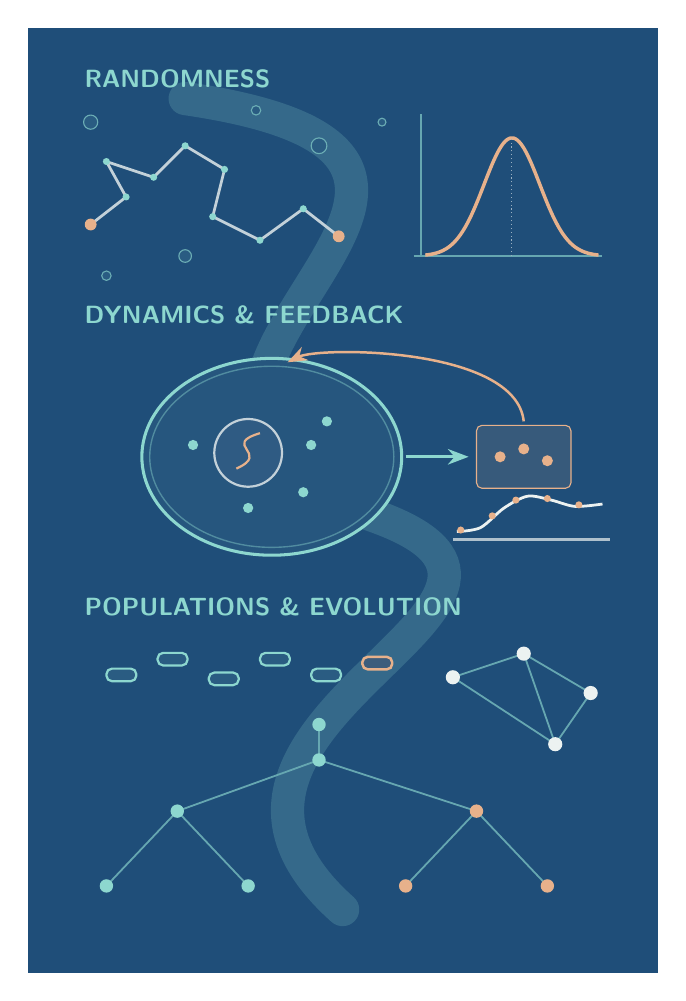
\begin{tikzpicture}[x=1cm,y=1cm,>=Stealth,
  every node/.style={font=\small,text=ivory},
  dot/.style={circle,inner sep=0pt,minimum size=3.5pt,fill=aqua},
  link/.style={draw=aqua!65!navy,line width=0.65pt},
  trace/.style={draw=ivory!80!navy,line width=1.0pt,line cap=round}]
\path[use as bounding box] (0,0) rectangle (8,12);
\fill[navy] (0,0) rectangle (8,12);
% A common thread connects fluctuations, feedback, and evolution.
\draw[draw=aqua!20!navy,line width=12pt,line cap=round]
  (2.0,11.1) .. controls (7.5,10.3) and (0.0,7.4) .. (4.4,5.8)
  .. controls (7.5,4.7) and (1.3,3.2) .. (4.0,0.8);

% Molecular noise: a discrete random trajectory, scattered particles,
% and a schematic distribution (not fitted or measured data).
\node[anchor=west,font=\small\sffamily\bfseries,text=aqua] at (0.6,11.35) {RANDOMNESS};
\draw[trace] (0.8,9.5)--(1.25,9.85)--(1.0,10.3)--(1.6,10.1)
  --(2.0,10.5)--(2.5,10.2)--(2.35,9.6)--(2.95,9.3)
  --(3.5,9.7)--(3.95,9.35);
\foreach \x/\y in {0.8/9.5,1.25/9.85,1.0/10.3,1.6/10.1,2/10.5,
  2.5/10.2,2.35/9.6,2.95/9.3,3.5/9.7,3.95/9.35}
  \fill[aqua] (\x,\y) circle (0.045);
\fill[copper] (0.8,9.5) circle (0.075);
\fill[copper] (3.95,9.35) circle (0.075);
\foreach \x/\y/\r in {0.8/10.8/.09,2.9/10.95/.06,3.7/10.5/.1,
  1.0/8.85/.06,2.0/9.1/.08,4.5/10.8/.05}
  \draw[aqua!70!navy,fill=aqua!10!navy] (\x,\y) circle (\r);
\draw[link] (4.9,9.1)--(7.3,9.1);
\draw[link] (5.0,9.1)--(5.0,10.9);
\draw[copper,line width=1.25pt,smooth,domain=5.05:7.25,samples=50]
  plot (\x,{9.1+1.5*exp(-4*(\x-6.15)^2)});
\draw[ivory!60!navy,densely dotted] (6.15,9.1)--(6.15,10.6);

% Cellular mechanism: a membrane/nucleus, a protein-production source,
% and an explicit feedback loop.
\node[anchor=west,font=\small\sffamily\bfseries,text=aqua] at (0.6,8.35) {DYNAMICS \& FEEDBACK};
\draw[fill=aqua!6!navy,draw=aqua,line width=1.1pt]
  (3.1,6.55) ellipse (1.65 and 1.25);
\draw[draw=aqua!45!navy,line width=0.5pt]
  (3.1,6.55) ellipse (1.55 and 1.15);
\draw[fill=ivory!8!navy,draw=ivory!80!navy,line width=0.8pt]
  (2.8,6.6) circle (0.43);
\draw[copper,line width=0.8pt] (2.65,6.4) .. controls (3.1,6.6) and
  (2.45,6.7) .. (2.95,6.85);
\foreach \x/\y in {2.1/6.7,3.5/6.1,3.8/7.0,2.8/5.9,3.6/6.7}
  \fill[aqua] (\x,\y) circle (0.065);
\node[draw=copper,fill=copper!12!navy,rounded corners=2pt,
  minimum width=12mm,minimum height=8mm] (protein) at (6.3,6.55) {};
\foreach \x/\y in {6.0/6.55,6.3/6.65,6.6/6.5}
  \fill[copper] (\x,\y) circle (0.07);
\draw[->,aqua,line width=1pt] (4.8,6.55)--(5.6,6.55);
\draw[->,copper,line width=0.9pt] (6.3,7.0)
  .. controls (6.2,7.95) and (3.7,7.95) .. (3.3,7.75);
\draw[ivory!70!navy,line width=0.8pt] (5.4,5.5)--(7.4,5.5);
\draw[ivory,line width=1.0pt,smooth]
  plot coordinates {(5.45,5.6)(5.75,5.65)(6.05,5.9)(6.35,6.05)(6.65,6.0)(6.95,5.92)(7.3,5.95)};
\foreach \x/\y in {5.5/5.62,5.9/5.8,6.2/6.0,6.6/6.02,7.0/5.94}
  \fill[copper] (\x,\y) circle (0.045);

% Populations, mutation and branching, and interaction networks.
\node[anchor=west,font=\small\sffamily\bfseries,text=aqua] at (0.6,4.65) {POPULATIONS \& EVOLUTION};
\foreach \x/\y in {1.0/3.7,1.65/3.9,2.3/3.65,2.95/3.9,3.6/3.7}
  \draw[aqua,fill=aqua!10!navy,rounded corners=2pt,line width=0.8pt]
    (\x,\y) rectangle +(0.38,0.16);
\draw[copper,fill=copper!15!navy,rounded corners=2pt,line width=0.9pt]
  (4.25,3.85) rectangle +(0.38,0.16);
\draw[link] (5.4,3.75)--(6.3,4.05)--(7.15,3.55)--(6.7,2.9)--(5.4,3.75)
  (6.3,4.05)--(6.7,2.9);
\foreach \x/\y in {5.4/3.75,6.3/4.05,7.15/3.55,6.7/2.9}
  \fill[ivory] (\x,\y) circle (0.09);
\draw[link] (3.7,3.15)--(3.7,2.7)--(1.9,2.05)
  (3.7,2.7)--(5.7,2.05)
  (1.9,2.05)--(1.0,1.1) (1.9,2.05)--(2.8,1.1)
  (5.7,2.05)--(4.8,1.1) (5.7,2.05)--(6.6,1.1);
\foreach \x/\y in {3.7/3.15,3.7/2.7,1.9/2.05,1/1.1,2.8/1.1}
  \fill[aqua] (\x,\y) circle (0.085);
\foreach \x/\y in {5.7/2.05,4.8/1.1,6.6/1.1}
  \fill[copper] (\x,\y) circle (0.085);
\end{tikzpicture}
\end{document}
